\documentclass{scrartcl}
\usepackage[utf8]{inputenc}
\usepackage{hyperref}
\usepackage{url}
\usepackage{natbib}
\usepackage{graphicx}
\usepackage{float}
\usepackage{cleveref} % this must be the last package to be loaded

\newcommand{\emailaddr}[1]{\href{mailto:#1}{\texttt{#1}}}

\title{\LARGE
    Dok \\
    \large A Distributed, Real-Time Collaborative Document Editor
}
\subtitle{Final Report for the Distributed Systems Course 2025/2026}

\author{
    Lorenzo Tosi \\ \emailaddr{lorenzo.tosi10@studio.unibo.it}
    \and
    Alessandro Stefani \\ \emailaddr{author2@gmail.com}
}

\date{\today}

\begin{document}

\maketitle

\begin{abstract}
Dok is a distributed, real-time collaborative document editing platform implemented as a
web application. It allows multiple users to create, share, and simultaneously edit text
documents. The system is built on a client--server architecture
in which the backend is horizontally scaled across two \textbf{Node.js/Express} server instances,
load-balanced by an \textbf{Nginx} reverse proxy. Real-time collaboration is achieved through
\textbf{Yjs} Conflict-free Replicated Data Types (CRDTs) transported over \textbf{Socket.io}
WebSocket connections; cross-instance event propagation is coordinated via a shared \textbf{Redis}
Pub/Sub adapter, which also enables cluster-wide user-presence tracking. Persistent state is stored
in a \textbf{MongoDB} document database. Documents are organised in folders and can be
made public or private, with sharing policies (\textit{viewer}, \textit{commenter},
\textit{editor}) enforced through \textbf{JWT}-based authentication and role-based access control. An administrative dashboard provides real-time platform-wide
statistics, audit trails, user presence information, and site-access logs. The entire infrastructure
is containerised with \textbf{Docker Compose}, making deployment reproducible with a single command.
\end{abstract}

\section*{Disclaimer}

During the preparation of this work, the author(s) used an AI-assisted coding assistant to support code scaffolding, refactoring, and the drafting of parts of this report.

After using this tool/service,
the author(s) reviewed and edited the content as needed
and take(s) full responsibility for the content of the final report/artifact.

\section{Concept}\label{concept}

\subsection{Type of Product}

Dok is a \textbf{web application with a graphical user interface}, accessible from any modern
browser without additional software installation. It combines a single-page application (SPA)
frontend, built with Vue~3 and Vite, with a horizontally scalable REST and WebSocket backend.

\subsection{Use-Case Description}

Dok targets teams of knowledge workers---students, researchers, and professionals---who need
to collaborate on written documents in real time from geographically dispersed locations.

\paragraph{What the system does.}
Users create rich-text documents (formatted paragraphs, headings, inline styling) and folders
to organise them. They can keep documents private, publish them to a global feed, or share them
selectively with other registered users under a specific permission level. Multiple users who
have access to the same document can edit it concurrently: their changes converge automatically
through CRDT semantics, and their cursor positions are broadcast live to collaborators. Inline
comments allow asynchronous annotation without disrupting the editing flow. An integrated AI
assistant (backed by Google Gemini) can rewrite any selected passage following a free-text
instruction. An administrator role provides platform-wide oversight: real-time user-presence,
per-user file-system trees, usage statistics, audit logs of document accesses and modifications,
and site-access logs.

\paragraph{Where and how users interact.}
Users interact exclusively through a browser-based SPA. They may be physically anywhere; the
platform is designed with network-distributed access in mind. Authenticated users access private
and shared content; unauthenticated visitors can read public documents and browse the public
dashboard.

\paragraph{User roles.}
Three end-user roles exist: \textit{Administrator} (first registered user is automatically
promoted), \textit{Authenticated User}, and \textit{Guest} (unauthenticated).
Document-level collaboration roles further distinguish \textit{owner}, \textit{editor},
\textit{commenter}, and \textit{viewer}.

\paragraph{Data stored.}
The system stores user accounts, documents (rich-text content serialised both as Yjs binary
state and Tiptap JSON), folders, comments, inter-user sharing metadata, per-document audit
logs, site-access logs, and real-time notifications.

\subsection{Why Distribution Is Needed}

Distribution addresses several independent needs:

\begin{itemize}
  \item \textbf{Concurrency and real-time collaboration.} Multiple users may edit the same
  document simultaneously. A single-process server would create a bottleneck and a single
  point of failure; horizontal scaling across multiple server instances, coordinated by Redis,
  removes both obstacles.
  \item \textbf{Fault tolerance.} Running at least two backend replicas behind a load balancer
  ensures that the failure of one instance does not render the service unavailable.
  \item \textbf{Resource sharing.} All backend instances share a single MongoDB database and a
  single Redis broker, making the system's data consistent regardless of which replica serves a
  given request.
  \item \textbf{Scalability.} The Nginx hash-based routing combined with the Redis Pub/Sub
  adapter allows new backend instances to be added with minimal configuration changes.
\end{itemize}


\section{Requirements Elicitation and Analysis}\label{requirements}

\subsection{Glossary}

\begin{description}
  \item[Dok] The name of the platform and the informal term for a document managed within it.
  \item[CRDT] Conflict-free Replicated Data Type---a data structure that can be merged from
  multiple concurrent sources without conflicts.
  \item[Yjs state] The binary serialisation of a Yjs document, stored in MongoDB and used to
  restore in-memory state when a document room is created.
  \item[Room] A Socket.io room identified by a document ID; all collaborators of a document
  join this room.
  \item[Presence] Whether a registered user currently has at least one active WebSocket
  connection to any server instance.
  \item[Audit log] A record of a user's access or modification event on a document.
\end{description}

\subsection{Functional Requirements}

\begin{enumerate}
  \item[\textbf{FR-1}] \textbf{User Registration and Authentication.}
  The system shall allow a visitor to register with email, first name, last name, and password.
  Subsequent logins shall return a JWT. The first registered user shall automatically receive
  the \textit{Administrator} role.
  \textit{Acceptance criterion:} A POST to \texttt{/api/auth/register} returns HTTP~201 with a
  valid JWT; a duplicate email returns HTTP~409.

  \item[\textbf{FR-2}] \textbf{Document Lifecycle.}
  An authenticated user shall be able to create, rename, and delete documents. Public documents
  shall be visible to all (including guests); private documents shall be visible only to their
  owner and explicitly invited collaborators.
  \textit{Acceptance criterion:} CRUD operations on \texttt{/api/documents} succeed for
  authorised users and return HTTP~403/404 for unauthorised ones.

  \item[\textbf{FR-3}] \textbf{Folder Hierarchy.}
  Users shall be able to organise documents in nested folders with configurable visibility.
  \textit{Acceptance criterion:} Folders support a self-referential parent/child relationship;
  documents within a folder are filtered when querying with \texttt{parentId}.

  \item[\textbf{FR-4}] \textbf{Fine-Grained Document Sharing.}
  The document owner shall be able to share a document with any registered user by email,
  assigning a role of \textit{viewer}, \textit{commenter}, or \textit{editor}. Roles can
  later be updated or revoked.
  \textit{Acceptance criterion:} PUT \texttt{/api/documents/share} modifies the
  \texttt{sharedWith} array; the target user receives a real-time notification.

  \item[\textbf{FR-5}] \textbf{Real-Time Collaborative Editing.}
  Concurrent edits by multiple users to the same document shall converge without loss of data,
  using CRDT semantics. All collaborators shall see changes within sub-second latency.
  \textit{Acceptance criterion:} Two clients connected to \emph{different} server instances who
  join the same document room both receive the \texttt{crdt-update} events produced by the
  other (validated in \texttt{distributed.test.ts}).

  \item[\textbf{FR-6}] \textbf{Cursor Awareness.}
  Users editing a document shall see the live cursor positions and names of co-editors.
  \textit{Acceptance criterion:} Clients receive \texttt{awareness-update} events relayed by
  the server.

  \item[\textbf{FR-7}] \textbf{Comments.}
  Owners, editors, and commenters shall be able to add inline comments to a document. Owners
  and editors can delete any comment; the comment author can delete their own.
  \textit{Acceptance criterion:} Verified by the role-matrix tests in
  \texttt{comments.test.ts}.

  \item[\textbf{FR-8}] \textbf{AI Writing Assistance.}
  An authenticated editor/owner shall be able to select a passage and submit a free-text
  instruction. The system shall invoke Google Gemini 2.5 Flash and return the rewritten text.
  \textit{Acceptance criterion:} POST \texttt{/api/llm} returns a JSON with
  \texttt{originalText} and \texttt{rewrittenText}.

  \item[\textbf{FR-9}] \textbf{Real-Time Notifications.}
  Users shall receive in-app notifications (via WebSocket) when a document is shared with
  them, when their permissions change, or when a document they have access to is deleted.
  \textit{Acceptance criterion:} Notification documents are persisted in MongoDB; unread count
  is updated in real time.

  \item[\textbf{FR-10}] \textbf{Administrative Dashboard.}
  An administrator shall be able to view: all registered users with online/offline presence;
  per-user usage metrics (documents created, shared); a user's private/public file-system
  tree; per-document audit logs; global platform statistics; site-access logs. The
  administrator shall also be able to promote/demote user roles.
  \textit{Acceptance criterion:} Admin endpoints return HTTP~403 for non-admin tokens.

  \item[\textbf{FR-11}] \textbf{Automatic Document Persistence.}
  The system shall automatically save the Yjs document state to MongoDB when editing activity
  ceases (debounced 3-second timer) and unconditionally when the last collaborator leaves.
  \textit{Acceptance criterion:} Verified in \texttt{distributed.test.ts}.

  \item[\textbf{FR-12}] \textbf{API Documentation.}
  The backend shall expose interactive API documentation via Swagger UI at
  \texttt{/api-docs}.
  \textit{Acceptance criterion:} Verified in \texttt{swagger.test.ts}.
\end{enumerate}

\subsection{Non-Functional Requirements}

\begin{enumerate}
  \item[\textbf{NFR-1}] \textbf{Availability.} The service shall remain available to clients
  if one of the two backend instances crashes, relying on Nginx's upstream failure detection.

  \item[\textbf{NFR-2}] \textbf{Consistency of Collaborative State.} Concurrent edits to
  the same document shall always converge to an identical final state, irrespective of the
  order in which updates are applied, thanks to CRDT properties.

  \item[\textbf{NFR-3}] \textbf{Low Editing Latency.} Changes made by one collaborator shall
  be propagated to other clients with sub-second latency under normal network conditions.

  \item[\textbf{NFR-4}] \textbf{Scalability.} The architecture shall support the addition of
  further backend replicas without changes to application code.

  \item[\textbf{NFR-5}] \textbf{Security.} Passwords shall be stored as bcrypt hashes (cost
  factor~12). All protected endpoints shall require a valid JWT; admin endpoints shall
  additionally verify the \textit{ADMIN} role.

  \item[\textbf{NFR-6}] \textbf{Maintainability.} The codebase shall be modular (controllers,
  services, models, socket handlers) and fully typed with TypeScript.
\end{enumerate}

\subsection{Implementation Constraints}

\begin{enumerate}
  \item[\textbf{IC-1}] The backend shall be implemented in \textbf{TypeScript} on
  \textbf{Node.js}, chosen for the ecosystem's excellent WebSocket support and the team's
  proficiency.
  \item[\textbf{IC-2}] The frontend shall be a \textbf{Vue~3} SPA, chosen for its reactive
  component model and first-class TypeScript integration.
  \item[\textbf{IC-3}] Real-time collaboration shall be built on \textbf{Yjs} CRDTs, the
  de-facto standard for operation-based collaborative editing without a central OT server.
  \item[\textbf{IC-4}] The entire backend stack shall be containerised with \textbf{Docker}
  to enable one-command deployment and reproducible environments.
  \item[\textbf{IC-5}] The AI feature shall use the \textbf{Google Gemini} API
  (\texttt{gemini-2.5-flash} model), requiring a valid \texttt{GEMINI\_API\_KEY} environment
  variable.
\end{enumerate}

\subsection{Relevant Distributed System Features}
\label{ds-features}

\paragraph{Transparency.}
Access, location, and replication transparency are important. Clients connect to a single
Nginx endpoint and are unaware of which backend instance serves their requests. The Redis
adapter makes socket rooms appear global; a client on server~1 receives events emitted by
server~2 without any application-level code change.

\paragraph{Fault tolerance and availability.}
Two backend replicas guarantee that a single-instance crash does not interrupt the service.
A 3-second grace period in the \texttt{PresenceManager} avoids misclassifying brief network
drops as permanent disconnections (network flap handling). The debounced save mechanism and
the unconditional flush on last-client-leave provide durability even if a server crashes
mid-session.

\paragraph{Scalability.}
The hash-consistent routing policy in Nginx routes all WebSocket connections for the same
document to the same backend instance (based on the \texttt{documentId} query parameter),
minimising unnecessary Redis roundtrips. Additional instances can be added to the
\texttt{upstream} block and the Docker Compose file.

\paragraph{Security and trust.}
Passwords are bcrypt-hashed, all API access is JWT-gated, and document-level RBAC enforces
four distinct permission levels. Admin-only endpoints are double-guarded by both the
\texttt{requireAuth} and \texttt{requireAdmin} middlewares.

\paragraph{Resource sharing.}
MongoDB and Redis are shared singletons across all backend replicas, providing a single
authoritative state for documents, users, and socket room membership.

\paragraph{Openness and interoperability.}
The REST API is documented with OpenAPI/Swagger, enabling third-party integration. The
Tiptap JSON format stored alongside the Yjs binary state allows export to standard rich-text
formats in future integrations.

\paragraph{Performance and concurrency.}
Yjs CRDTs handle concurrent writes without locking. MongoDB's optimistic concurrency
(the \texttt{optimisticConcurrency} flag on Folder and Document schemas) handles rare
database-level write conflicts. Audit-log aggregation (character counting) is batched in
memory and flushed lazily to avoid per-keystroke database writes.

\paragraph{Economy.}
The use of free-tier-compatible managed services (MongoDB, Redis) in the Docker Compose
setup keeps operational costs minimal for small deployments.


\section{Design}\label{design}

This chapter presents the strategies used to meet the requirements of \cref{requirements}.

\subsection{Architecture}\label{architecture}

Dok follows a classic \textbf{client--server, three-tier architecture} with a \emph{stateless application tier} and a \emph{shared state tier}:

\begin{itemize}
  \item \textbf{Presentation tier} --- a Vue 3 SPA running in the user's browser.
  \item \textbf{Application tier} --- one or more identical Node.js processes exposing both a REST API (Express) and a WebSocket endpoint (Socket.IO). This tier is \emph{stateless with respect to HTTP} but holds \emph{ephemeral session state} for the documents currently being edited (the in-memory Yjs documents).
  \item \textbf{State tier} --- a single MongoDB instance for persistence and a single Redis instance used as a Socket.IO pub/sub backbone.
\end{itemize}

The chosen style is a \emph{service-oriented, horizontally scalable monolith}: each backend instance is a replica of the same application, and the load balancer distributes requests among them. This style is appropriate because the dominant workload (live editing) is interactive and benefits from low-latency, sticky connections, while the REST workload is stateless and trivially parallelisable. Distribution is achieved by \emph{replication of the application code} rather than by partitioning the domain across microservices, which keeps the system simple while still allowing scale-out.

A central design decision is \textbf{where edit consistency is enforced}. Rather than using a central sequencer or operational-transform server, Dok delegates consistency to a CRDT: each client and the server hold a replica of the document's Yjs document, and updates commute. This removes the need for distributed locking and is the key enabler of location transparency.

\subsection{Infrastructure}\label{infrastructure}

The infrastructural components, as defined in the \texttt{docker-compose.yml}, are:

\begin{itemize}
  \item \textbf{Nginx} (\texttt{nginx:alpine}): A single entry point on port~3000.
  It terminates incoming HTTP and WebSocket connections and forwards them to the upstream
  cluster. WebSocket upgrade headers (\texttt{Upgrade}, \texttt{Connection}) are forwarded
  explicitly. The real client IP is passed via \texttt{X-Real-IP}.
  \item \textbf{backend1} and \textbf{backend2}: two replicas of the Node.js application, built from \texttt{server/Dockerfile}. They are intentionally identical to demonstrate horizontal scaling.
  \item \textbf{mongo} (\texttt{mongo:latest}): the single shared document database, exposed on port 27017.
  \item \textbf{redis} (\texttt{redis:alpine}): the pub/sub broker for Socket.IO cross-instance messaging, exposed on port 6379.
\end{itemize}

\textbf{Distribution over the network.} In the reference deployment all containers run on a single Docker host (single datacenter, single network). However, the topology is designed so that any subset of these components could be relocated: the backends are stateless and discover the database and broker purely through environment variables (\texttt{MONGO\_URI}, \texttt{REDIS\_URL}), so placing MongoDB or Redis on another host or a managed cloud service requires no code change.

\textbf{Component naming and discovery.} Discovery is centralised and static: Docker Compose's internal DNS resolves service names (\texttt{backend1}, \texttt{backend2}, \texttt{mongo}, \texttt{redis}) to their container IP addresses. Nginx references the two backends by name in its \texttt{upstream} block; the Node.js processes reference MongoDB and Redis by URL. There is no dynamic service registry because the set of backends is fixed and small.

\textbf{Routing strategy.} This is one of the most important infrastructural choices. The \texttt{nginx.conf} defines a single upstream and uses the \texttt{hash} directive with the \texttt{consistent} option:

\begin{quote}
\begin{verbatim}
map $arg_documentId $route_key {
    "~^.+$"  $arg_documentId;
    default  $remote_addr;
}
upstream websocket_cluster {
    hash $route_key consistent;
    server backend1:3000;
    server backend2:3000;
}
\end{verbatim}
\end{quote}

The hash key is the \texttt{documentId} query parameter when present, and the client IP otherwise. This implements \textbf{application-aware consistent hashing}: all clients editing the \emph{same} document are routed to the \emph{same} backend, which is where that document's live Yjs replica resides. Consistent hashing (rather than round-robin) is chosen so that adding or removing a backend only re-maps a fraction of the keyspace, minimising disruption. Pure stateless REST calls (no \texttt{documentId}) fall back to client-IP hashing for a rough load balance. Nginx is configured for WebSocket upgrade (\texttt{proxy\_http\_version 1.1} plus the \texttt{Upgrade}/\texttt{Connection} headers), which is required for Socket.IO long-lived connections.

\begin{figure}[H]
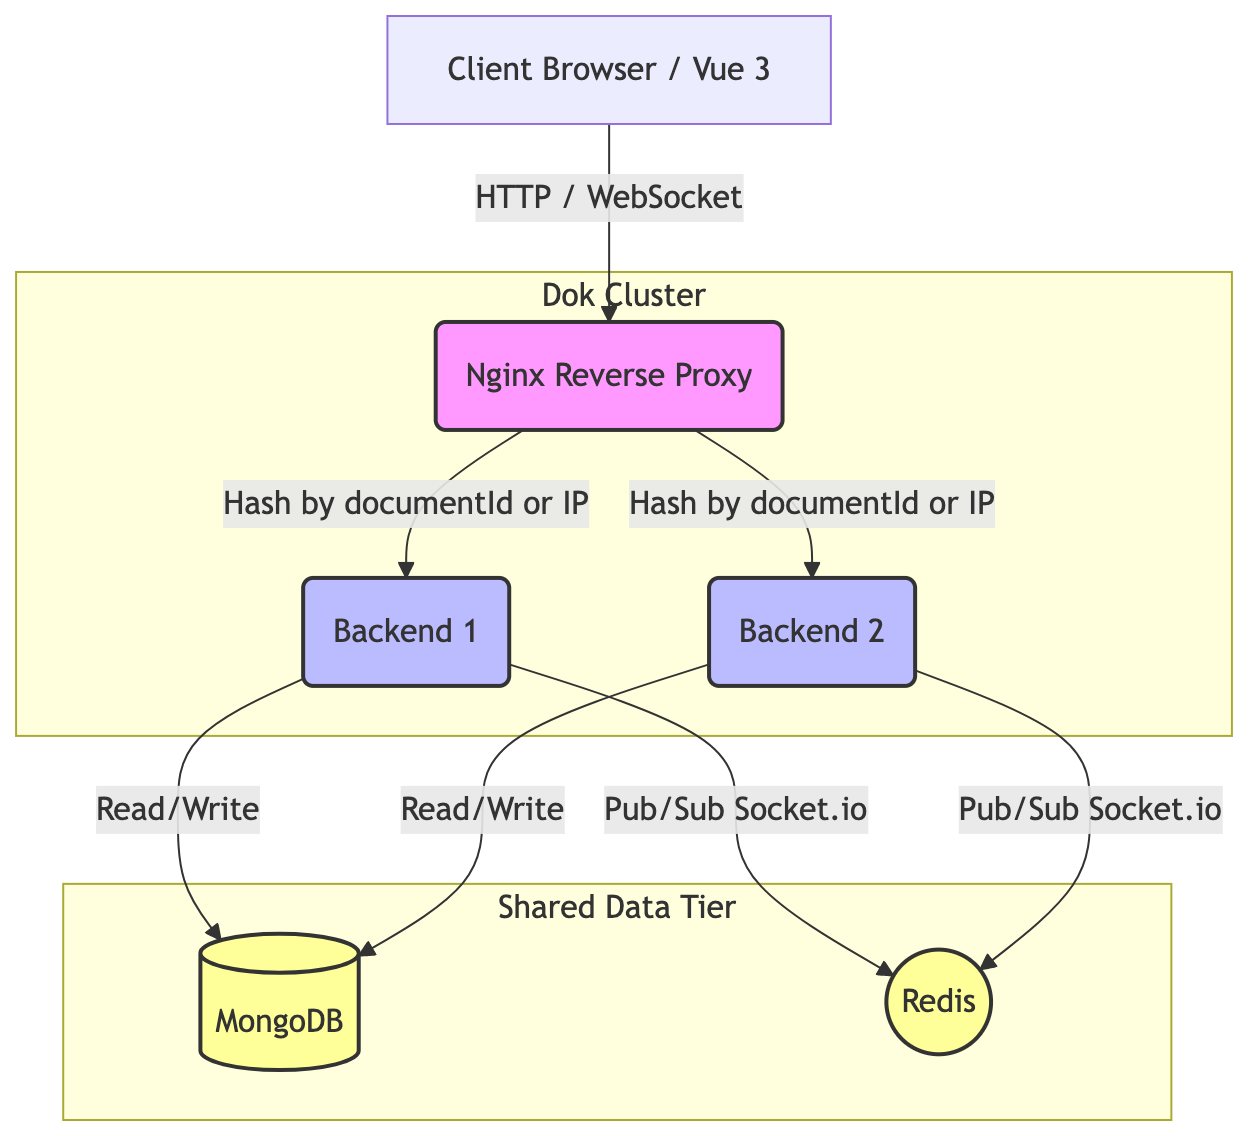
\includegraphics[scale=0.3]{diagrammi/arch.png}
\caption{Component and Deployment Diagram.}
\centering
\end{figure}



\subsection{Modelling}\label{modelling}

\textbf{Domain entities.} The persisted domain model, expressed as Mongoose schemas, consists of:

\begin{itemize}
  \item \texttt{User} --- \texttt{email} (unique), \texttt{passwordHash}, \texttt{role} (\texttt{USER}|\texttt{ADMIN}), \texttt{firstName}, \texttt{lastName}, \texttt{lastSeen}, plus timestamps.
  \item \texttt{Document} --- \texttt{title}, \texttt{ownerId}, \texttt{folderId}, \texttt{visibility} (\texttt{private}|\texttt{public}), an array \texttt{sharedWith} of \{\texttt{userId}, \texttt{role}\}, an array \texttt{comments} of \{\texttt{userId}, \texttt{content}\}, the binary \texttt{yjsState} (the serialised CRDT), and a \texttt{tiptapJson} projection for rendering.
  \item \texttt{Folder} --- \texttt{name}, \texttt{ownerId}, \texttt{parentId}, \texttt{visibility}.
  \item \texttt{Notification} --- \texttt{recipient}, \texttt{sender}, \texttt{type} (\texttt{SHARE}|\texttt{PERM\_CHANGE}|\texttt{DOCUMENT\_DELETE}|\texttt{SYSTEM}), \texttt{title}, \texttt{message}, \texttt{documentId}, \texttt{read}, \texttt{link}.
  \item \texttt{AuditLog} --- \texttt{documentId}, \texttt{userId}, \texttt{type} (\texttt{access}|\texttt{modification}), \texttt{charactersInserted}.
  \item \texttt{SiteAccessLog} --- \texttt{userId}, \texttt{loginAt}, \texttt{logoutAt}, \texttt{ipAddress}.
\end{itemize}

\textbf{In-memory state.} Alongside the persisted model, each backend holds a \texttt{Map<string, ActiveDocState>} of documents currently being edited. Each entry contains the live \texttt{Y.Doc}, a \texttt{clientsCount}, a debounced \texttt{saveTimeout}, and a \texttt{pendingUserChars} map used to aggregate modification audit logs. This ephemeral state is the unit that is pinned to a single backend by the consistent-hashing router.

\textbf{Mapping entities to infrastructure.} Persistent entities live in the shared MongoDB, accessible from every backend. The live editing state (the CRDT) lives in the memory of exactly one backend per document --- the one selected by Nginx. Awareness (caret positions, colour, user name) is ephemeral and not persisted; it flows only through the socket layer.

\textbf{Domain events.} Examples include: \emph{user registered/logged in}, \emph{document created/deleted/renamed}, \emph{document shared/unshared}, \emph{comment added/deleted}, \emph{user joined/left a document}, \emph{role changed}.

\textbf{Messages.} The system exchanges two families of messages:

\begin{itemize}
  \item \textbf{REST commands/queries} (HTTP/JSON): \texttt{POST /api/auth/register}, \texttt{POST /api/documents}, \texttt{PUT /api/documents/share}, \texttt{POST /api/documents/:id/comments}, the admin endpoints, etc. These are the source of truth for non-collaborative state changes.
  \item \textbf{Socket.IO events}: \texttt{join-document}, \texttt{sync-document}, \texttt{crdt-update}, \texttt{awareness-update}, \texttt{leave-document}, plus notification events (\texttt{new-notification}, \texttt{document-renamed}, \texttt{presence\_update}, \texttt{new\_audit\_log}, \dots). These carry the live, collaborative traffic.
\end{itemize}


\begin{figure}[H]
    \centering
    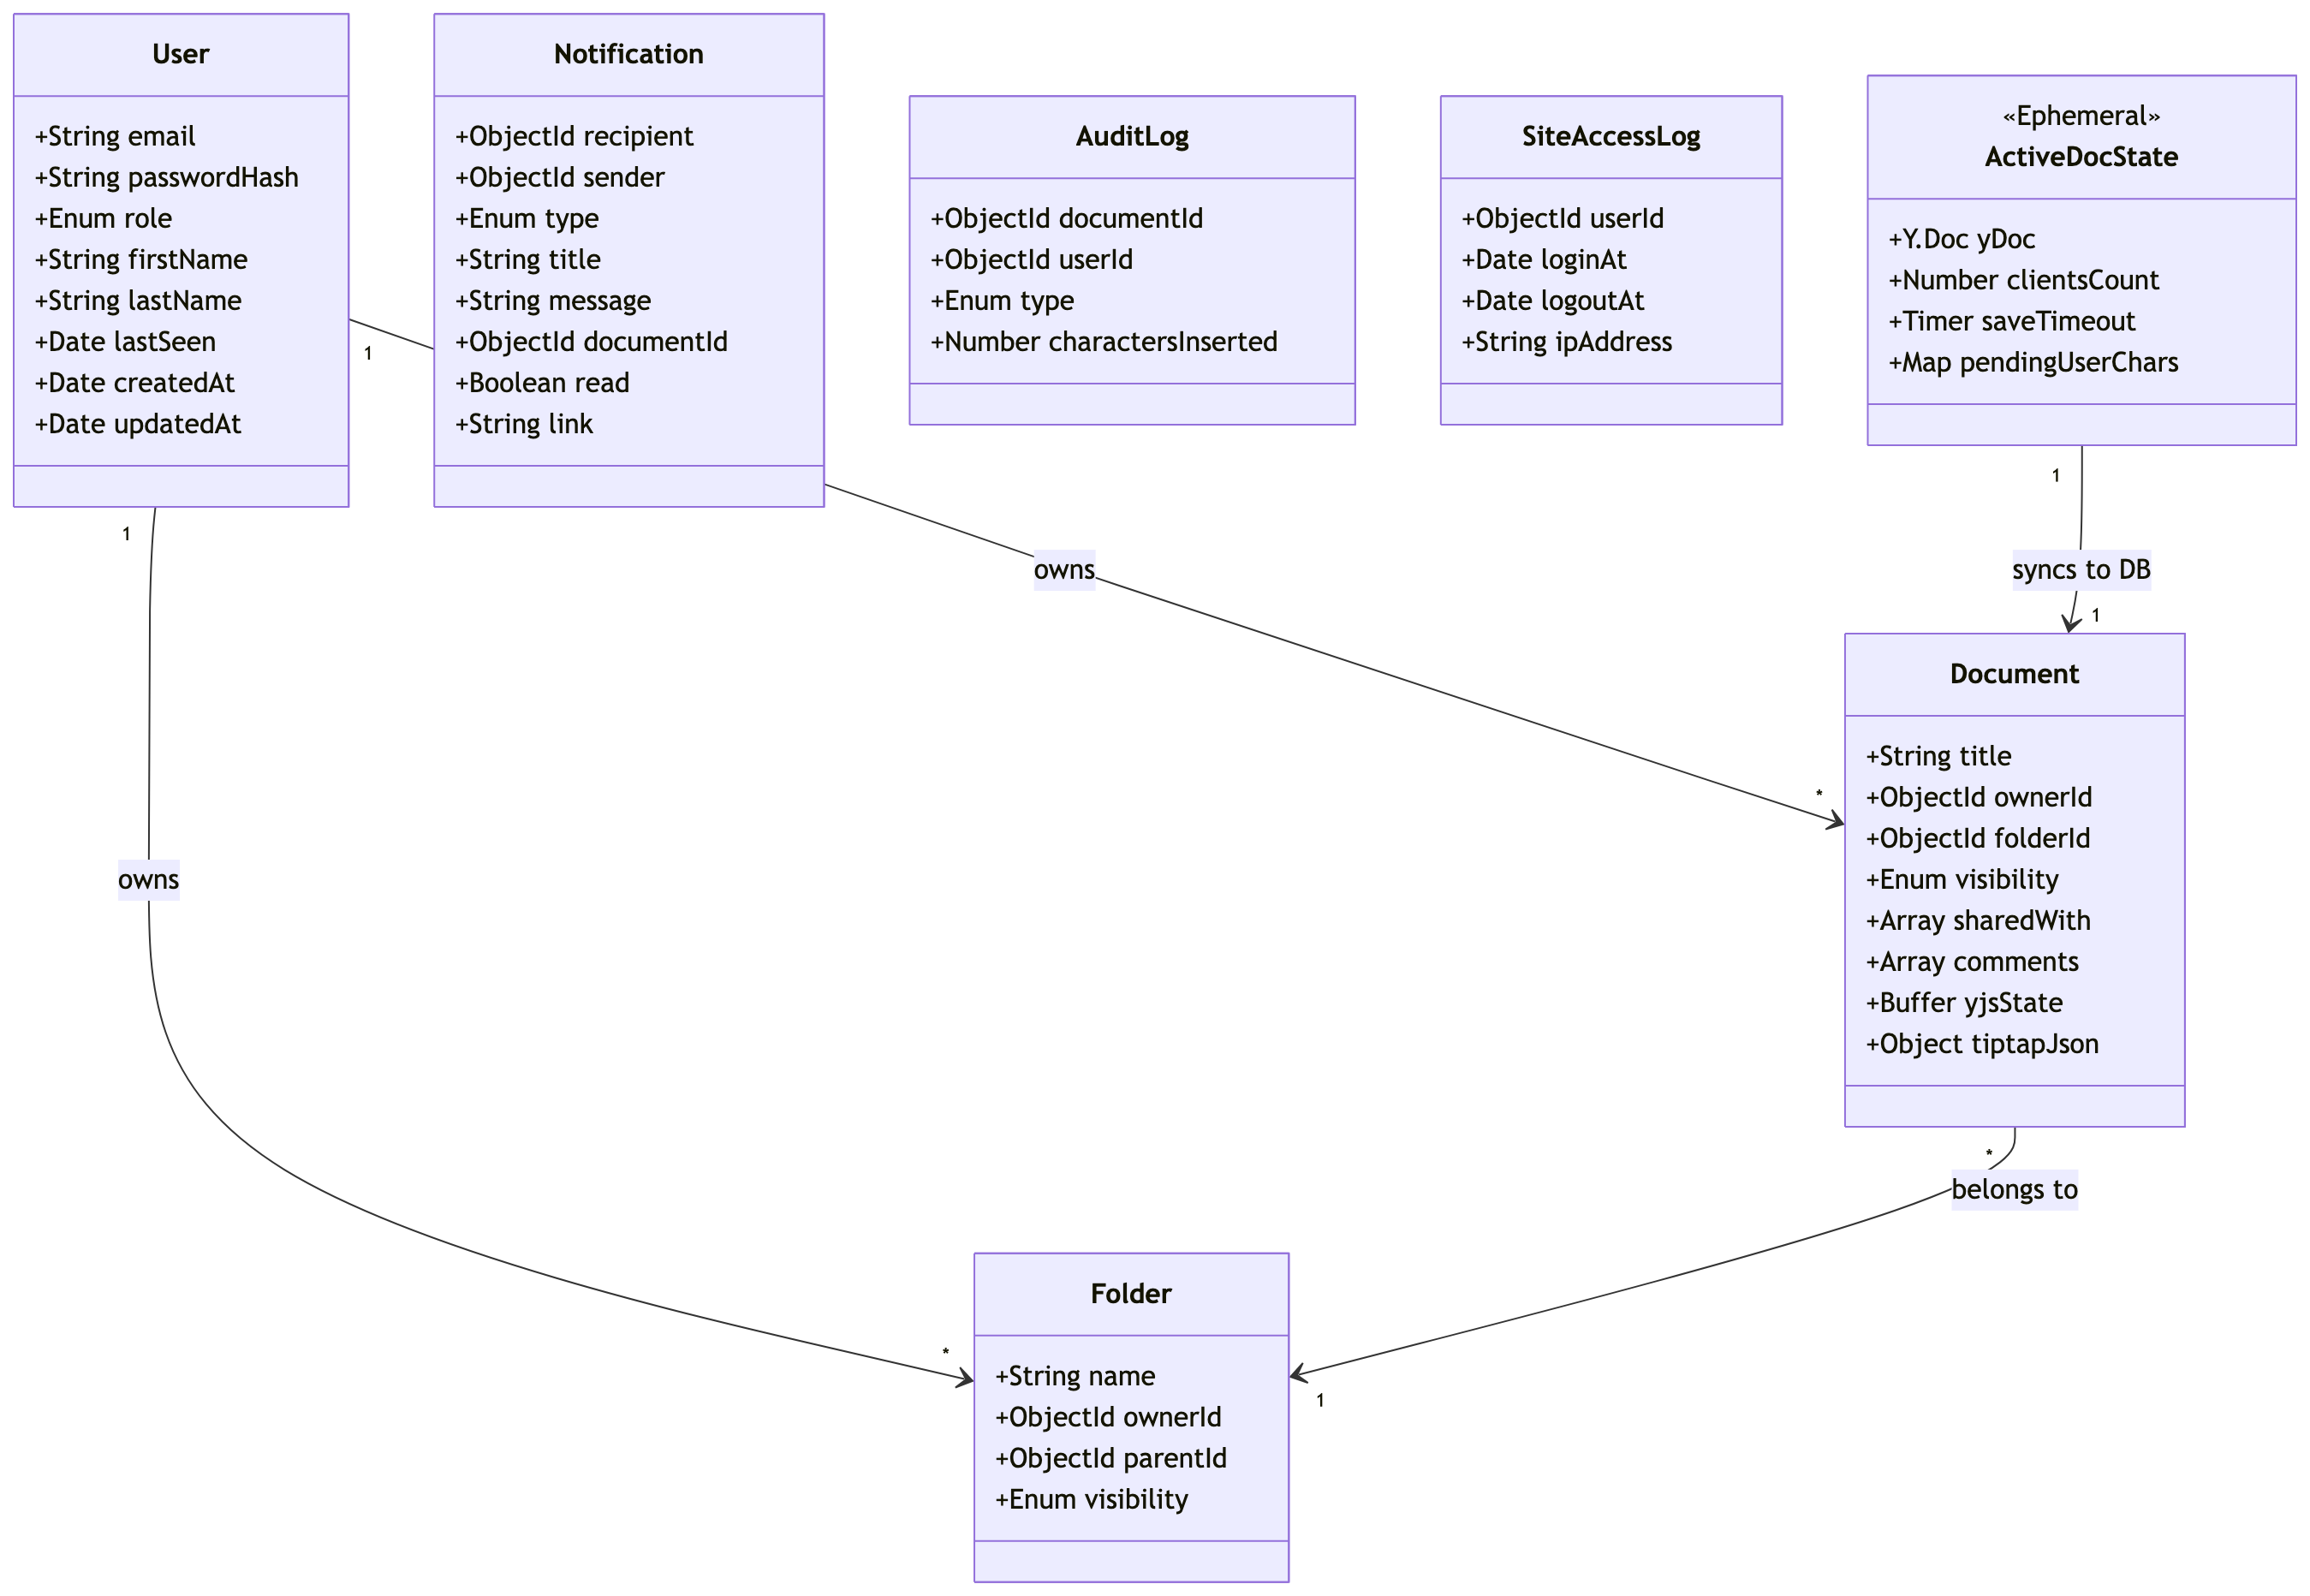
\includegraphics[width=12cm, height=6.5cm]{diagrammi/class.png}
    \caption{Class diagram.}
\end{figure}


\subsection{Interaction}\label{interaction}

Two distinct interaction patterns coexist, chosen to match the nature of each operation:

\begin{itemize}
  \item \textbf{Request--response (synchronous, over HTTP/JSON).} Used for operations that change durable state and require an immediate success/failure acknowledgement: authentication, CRUD on documents and folders, sharing, commenting, and all administrative actions. This pattern is stateless and therefore trivially load-balanced across backends by Nginx.
  \item \textbf{Publish--subscribe / event streaming (asynchronous, over WebSocket).} Used for the live editing session and for real-time notifications. Within a single backend, the classic Socket.IO room abstraction is used: joining a document means joining a room named after the document id, and \texttt{socket.to(room).emit(...)} fans updates out to the other participants. \emph{Across} backends, the Socket.IO Redis adapter transparently relays emissions through Redis pub/sub channels, so a client connected to backend2 receives an update emitted on backend1 as if they were on the same process.
\end{itemize}

The lifecycle of a collaborative editing session is the canonical interaction:

\begin{enumerate}
  \item The client opens a document, opening a Socket.IO connection whose URL carries \texttt{?documentId=...}; Nginx hashes this id and routes the connection to a fixed backend.
  \item The client emits \texttt{join-document}; the server loads (or reuses) the in-memory CRDT, applies any persisted binary state, joins the socket room, and replies with \texttt{sync-document} containing the full encoded CRDT state.
  \item On each local edit the client emits \texttt{crdt-update} with the binary update; the server applies it to its CRDT (tagging the transaction origin with the user id for auditing) and re-broadcasts it to the room via \texttt{socket.to(documentId).emit(...)}; the Redis adapter forwards it to other backends if needed.
  \item Awareness updates (caret position, selection, user identity) flow symmetrically through \texttt{awareness-update}.
  \item On \texttt{leave-document} or \texttt{disconnecting}, the server decrements the client count; when it reaches zero the final state is flushed to MongoDB and the in-memory CRDT is garbage-collected.
\end{enumerate}

\begin{figure}[H]
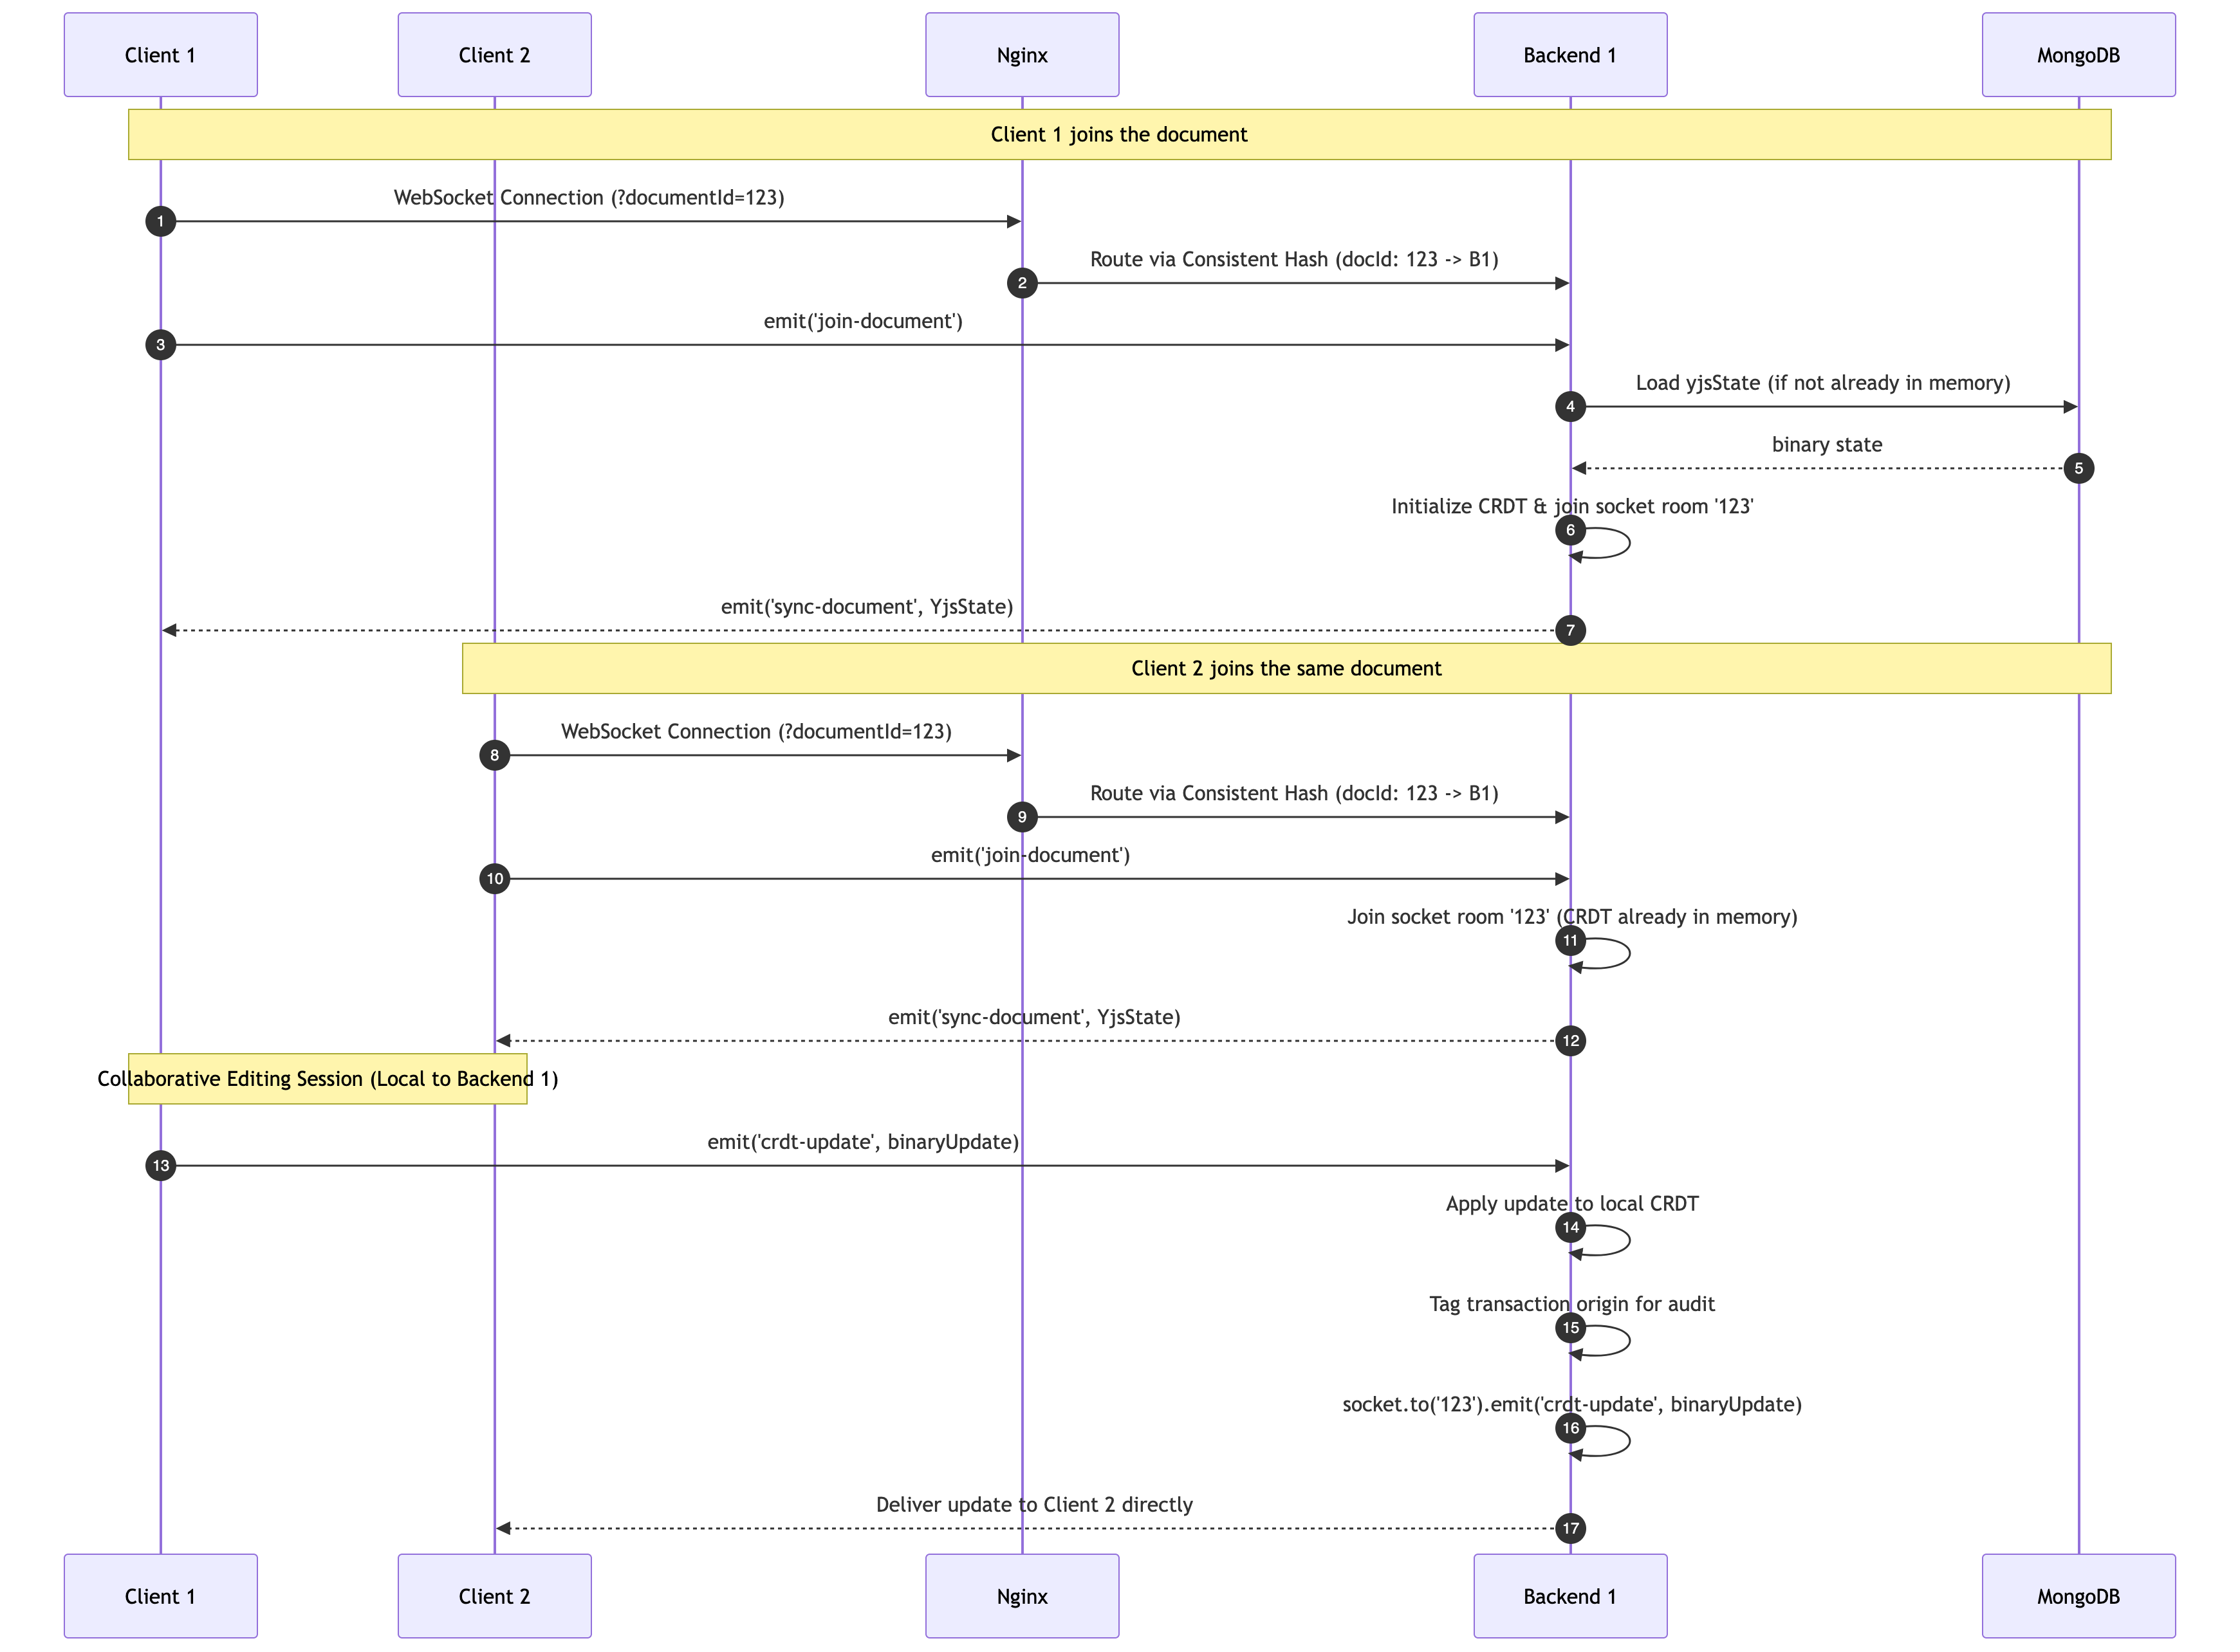
\includegraphics[scale=0.13]{diagrammi/edit.png}
\caption{Example of 2 user joining and editing the same document.}
\centering
\end{figure}


\paragraph{Real-time file-system event propagation.}
Beyond the collaborative editing channel, Redis plays a second, equally important role: it is the
backbone for propagating \emph{structural changes} to the file system in real time. When a user
performs an action that modifies the shared state of the dashboard---creating, renaming, or deleting
a document, or sharing/unsharing it with a collaborator---the service layer invokes the
\texttt{NotificationManager}, which emits targeted Socket.IO events to one or more rooms.
Because the Socket.IO Redis adapter is active, these emissions are transparently forwarded to
\emph{all} backend instances, so every connected client receives the update regardless of which
server instance hosts their WebSocket connection.

The rooms involved and the events emitted are:
\begin{itemize}
  \item \textbf{\texttt{global-dashboard}} --- receives \texttt{global-document-created},\\
  \texttt{global-document-renamed}, and \texttt{global-document-deleted} whenever a
  \emph{public} document changes. All clients watching the public feed join this room \\
  (via \texttt{join-public-dashboard}) and refresh their view without polling.

  \item \textbf{\texttt{user:\{id\}}} (private per-user room) --- receives
  \texttt{private-document-created},\\ \texttt{private-document-deleted},
  \texttt{document-renamed}, \texttt{document-shared},\\ \texttt{document-unshared},
  \texttt{new-notification}, and \texttt{role-changed}. Every authenticated client joins
  their own private room immediately on connection \\
  (\texttt{socket.join(`user:\$\{userId\}`)}), so the owner of a document sees their
  dashboard updated instantly when one of their private documents is renamed or deleted, and
  a collaborator's ``Shared with me'' panel updates immediately when a document is shared
  with them or revoked.

  \item \textbf{\texttt{\{documentId\}}} (document editing room) --- receives
  \texttt{document-renamed},\\ \texttt{document-shared}, \texttt{document-unshared} while
  users are actively inside the editor, so the title bar and the collaborator list react in
  real time without a page reload.

  \item \textbf{\texttt{admin:dashboard}} --- receives \texttt{presence\_update},
  \texttt{user\_metrics\_update}, and \\ \texttt{new\_audit\_log}. The administrator panel
  joins this room and displays live counters (documents created, shared) and the online/offline
  state of every user.
\end{itemize}

The entire notification chain is synchronous from the service layer's perspective: after each
mutating REST call completes (e.g., \texttt{PUT /api/documents/share}), the service calls
\texttt{NotificationManager.notifyDocumentShared(\ldots)}, which calls
\texttt{io.to(\ldots).emit(\ldots)} on the local Socket.IO server instance. The Redis adapter
serialises the emission and publishes it to the appropriate Redis channel; every other backend
instance subscribed to that channel delivers it to its locally connected clients. The result is
that the client who \emph{initiated} the REST action and the clients who are affected by it---even
if they are connected to \emph{different} backend instances---all observe the updated state within
milliseconds, without any polling.

\begin{figure}[H]
    \centering
    
\includegraphics[scale=0.09]{diagrammi/share.png}
    \caption{Example of real time creation of new document, sharing it and receiving the notification.}
\end{figure}

\subsection{Behaviour}\label{behaviour}

\textbf{Backend behaviour.} Each backend is event-driven and single-threaded (Node.js). Its components behave as follows:

\begin{itemize}
  \item \textit{Document handler} (stateful, per document). On \texttt{join-document} it lazily loads the CRDT from MongoDB and registers a deep observer on the Yjs XML fragment. The observer inspects each CRDT transaction's \texttt{origin} (which the server sets to the editing user's id when applying a remote update) and accumulates inserted characters per user into \texttt{pendingUserChars}; this provides attribution for the audit log without per-keystroke database writes. On every \texttt{crdt-update} it resets a 3-second debounce timer: when editing pauses for 3~seconds, the full binary state and the Tiptap JSON projection are persisted. This \emph{debounced persistence} is the main mechanism that keeps database write load proportional to \emph{editing sessions} rather than to \emph{keystrokes}, addressing the performance concern of \cref{ds-features}.
  \item \textit{Presence manager} (stateful, per user). On connection it joins a per-user room \texttt{user:<id>}; because the room is shared across backends through Redis, the count of sockets in the room is a cluster-wide online indicator. On disconnect it waits a 3-second \emph{grace period} before declaring the user offline: if a new connection appears within the window (a transient network flap or a device switch) the offline transition is cancelled. Only when the room is genuinely empty does it update \texttt{lastSeen} in the database and emit \texttt{presence\_update} to the admin room.
  \item \textit{Notification manager} (stateless facade over the socket instance). It is initialised
    once at startup with a reference to the Socket.IO \texttt{Server} object and exposes a set of
    domain-level methods called by the service layer after each mutating operation:
    \begin{itemize}
        \item \texttt{notifyDocumentCreated}.
        \item \texttt{notifyDocumentDeleted}.
        \item \texttt{notifyDocumentRenamed}.
        \item \texttt{notifyDocumentShared}.
        \item \texttt{notifyDocumentUnshared}.
        \item \texttt{notifyCommentAdded}.
        \item \texttt{notifyCommentDeleted}.
        \item \texttt{notifyAdminMetricsUpdate}.
        \item \texttt{notifyRoleChanged}.
    \end{itemize}
    Each method translates a domain event into one or more \texttt{io.to(room).emit(\ldots)} calls,
    routing the event to the correct set of recipients (a single user room, a document room, the
    global dashboard, or the admin dashboard). Because the Socket.IO Redis adapter is attached to the
    same \texttt{io} instance, every emission is automatically replicated across all backend instances:
    the \texttt{NotificationManager} is therefore completely stateless and instance-agnostic---it
    emits locally and Redis takes care of cluster-wide delivery.
  \item \textit{Auth middleware} (stateless). Validates the JWT on every protected HTTP route and on the socket handshake; for sockets, an absent token is tolerated (guest), while an invalid token is rejected.
\end{itemize}

\textbf{Who updates the state.} The single source of truth for a document's content is the in-memory CRDT on the owning backend; it is updated by the \texttt{crdt-update} handler and periodically checkpointed to MongoDB by the debounce/flush logic. All other durable state (users, folders, sharing, notifications, logs) is updated synchronously by the service layer in response to REST commands, against the shared MongoDB. Because the CRDT guarantees convergence, no component needs to coordinate with others to ``update the state correctly'' --- replicas simply apply commutative updates.


\begin{figure}[H]
    \centering
    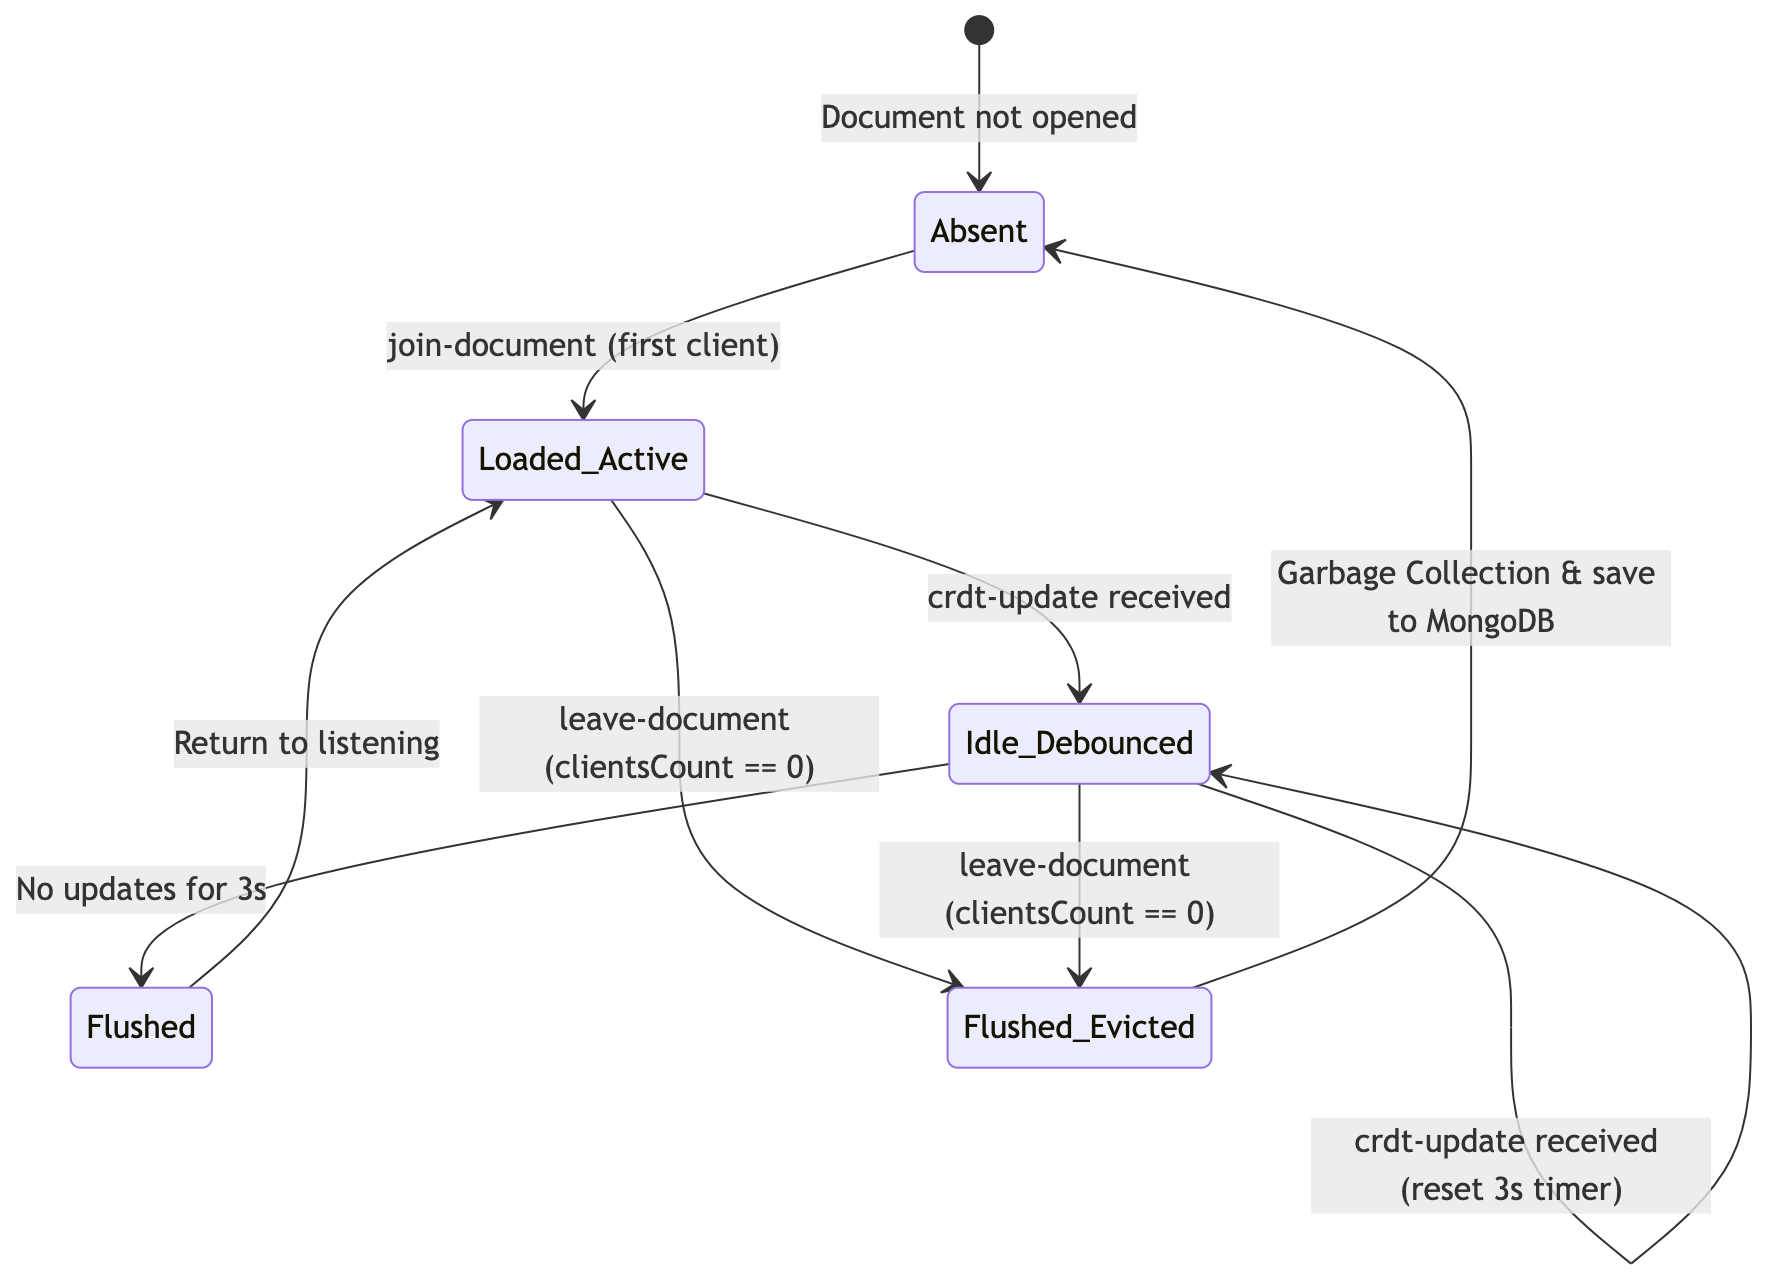
\includegraphics[scale=0.22]{diagrammi/states.png}
    \caption{Document lifecycle inside server.}
\end{figure}



\subsection{Data and Consistency Issues}\label{data-and-consistency-issues}

\paragraph{Persistent data.}
All domain entities are stored in MongoDB as BSON documents. The choice of a document store
is motivated by the document-centric nature of the application: each Dok naturally maps to a
MongoDB document with embedded comments and sharing metadata, avoiding expensive
JOIN-equivalent operations.

\paragraph{CRDT consistency.}
Document content is maintained as a Yjs \texttt{Y.Doc}. Yjs implements a LOGOOT-inspired
CRDT with vector-clock based causality. Because CRDT merges are commutative, associative,
and idempotent, concurrent edits from any number of clients always converge to the same
final state without requiring a central coordinator or Operational Transformation. The server
holds the canonical in-memory CRDT state for each active document and serialises it to
MongoDB on a periodic basis.

\paragraph{Optimistic concurrency.}
The \texttt{Document} and \texttt{Folder} Mongoose schemas use \\
\texttt{optimisticConcurrency: true}, which adds a \texttt{\_\_v} (version key) check on
\texttt{save()} to detect conflicting writes at the database level (analogous to optimistic
locking in relational databases). This guards against rare race conditions in HTTP endpoints
that read-then-modify a document.

\paragraph{Shared data between components.}
The \texttt{yjsState} field in MongoDB acts as the handoff point between instances. If a
client connects to instance~2 for a document that instance~1 last persisted, instance~2
loads the latest \texttt{yjsState} from MongoDB and reconstructs the \texttt{Y.Doc} from
scratch, correctly replaying all prior operations encoded in the binary snapshot.

\subsection{Fault-Tolerance}\label{fault-tolerance}

\paragraph{Replica redundancy.}
Two backend instances eliminate the single point of failure at the application server level.
If one instance crashes, Nginx's upstream health-check mechanism stops routing new
connections to it, and clients will reconnect to the surviving instance. The Redis adapter
state (room membership) reconstructs automatically as clients reconnect.

\paragraph{Grace period for network flap.}
The \texttt{PresenceManager.removeConnection} method waits 3~seconds before marking a user
offline and updating \texttt{lastSeen}. This handles transient network interruptions and
multi-tab scenarios: if the socket reconnects within the grace period, the user is never
declared offline.

\paragraph{Debounced persistence and flush-on-close.}
The dual save strategy (3-second debounce \emph{plus} unconditional flush when
\texttt{clientsCount} reaches zero) ensures that the maximum data loss window is bounded by
the debounce interval. Even a sudden server crash at most loses 3~seconds of edits for
documents that had active clients on that instance at the time of failure.

\paragraph{LLM retry logic.}
The \texttt{LLMEngine} retries failed Gemini API calls up to 3 times before surfacing an
error, tolerating transient network or rate-limit failures from the external API.

\paragraph{Error handling.}
Errors in background tasks (metric updates, sharing metric refreshes) are caught and logged
but do not propagate to the calling request, preventing auxiliary failures from disrupting
the primary user action.

\subsection{Availability}\label{availability}

\textbf{Caching.} There is intentionally little caching: the in-memory \texttt{activeDocuments} map is effectively a \emph{session cache} of live documents, present only on the owning backend. The \texttt{tiptapJson} projection persisted alongside the CRDT acts as a pre-computed rendering cache so that read-only opens do not need to run the Yjs$\rightarrow$Tiptap transformation.

\textbf{Load balancing.} Nginx performs load balancing with the consistent-hashing strategy described in \cref{infrastructure}. This simultaneously balances connection load and enforces session stickiness, which is what makes the single-replica-per-document design correct. For pure REST traffic (no \texttt{documentId}), client-IP hashing provides a fairer distribution.

\textbf{Network partitioning.} Because all backend instances share MongoDB and Redis, a partition between the two instances
would be detected by the Redis adapter (connection errors logged), but MongoDB reads/writes
from each instance would still succeed independently. The system makes no formal
partition-tolerance guarantees; it prioritises consistency and availability under the
assumption that intra-datacenter network partitions are rare.

\subsection{Security}\label{security}

\paragraph{Authentication.}
All protected REST endpoints require an \texttt{Authorization: Bearer \{JWT\}} header. The
Socket.io handshake passes the JWT via \texttt{socket.handshake.auth.token}. Tokens are
signed with the HS256 algorithm using a secret read from the \texttt{JWT\_SECRET} environment
variable (defaulting to a development placeholder that must be overridden in production).
Tokens expire after 24 hours.

\paragraph{Password security.}
The \texttt{User} model hashes passwords via a Mongoose pre-save hook using bcrypt with a
cost factor of~12. The \texttt{passwordHash} field has \texttt{select: false}, preventing
accidental exposure in query results.

\paragraph{Authorisation.}
Three layers of access control are enforced:
\begin{enumerate}
  \item \textbf{Endpoint-level RBAC}: \texttt{requireAuth} (any valid JWT) and
  \texttt{requireAdmin} (JWT with \texttt{role === ADMIN}) middleware guard route groups.
  \item \textbf{Document-level ownership checks}: Service methods verify \texttt{ownerId}
  or \texttt{sharedWith} membership before performing mutations.
  \item \textbf{Comment-level role checks}: Comment creation and deletion enforce the four
  document roles (owner, editor, commenter, viewer).
\end{enumerate}

\paragraph{Input validation.}
The \texttt{requireBodyField} and \texttt{validateMongoIdParam} middleware functions reject
malformed requests before they reach business logic.

\paragraph{Admin data masking.}
The \texttt{AdminService.getDocumentInfoForAdmin} method replaces the title of private
documents with the string ``Documento Riservato'', and strips \texttt{tiptapJson} and
\texttt{yjsState} from the response, ensuring that administrators cannot read the
\emph{content} of private documents they do not own.


\section{Implementation}\label{implementation}

\subsection{Network Protocols}

\begin{itemize}
  \item \textbf{HTTP/1.1} for REST API traffic. Nginx upgrades WebSocket connections via the
  \texttt{Upgrade} header mechanism.
  \item \textbf{WebSocket} (over HTTP/1.1 Upgrade) for all real-time communication, managed
  by Socket.io.
  \item \textbf{Redis RESP} (Redis Serialisation Protocol) for pub/sub communication between
  the Socket.io adapter clients and the Redis broker.
  \item \textbf{MongoDB Wire Protocol} for all database interactions.
\end{itemize}

\subsection{Data Representation}

\begin{itemize}
  \item \textbf{REST API}: All request and response bodies are JSON; Express's
  \texttt{express.json()} middleware handles parsing and serialisation.
  \item \textbf{Yjs CRDT state}: Transmitted over WebSocket as binary \texttt{Uint8Array}
  (encoded by \texttt{Y.encodeStateAsUpdate}); stored in MongoDB as a \texttt{Buffer} in
  the \texttt{yjsState} field.
  \item \textbf{Rich-text snapshot}: A Tiptap-compatible JSON document (\texttt{tiptapJson})
  is stored alongside the binary state for potential future use by read-only consumers.
  \item \textbf{JWT payload}: JSON object with \texttt{id} and \texttt{role} fields, signed
  with HS256.
\end{itemize}

\subsection{Database}

MongoDB is queried via \textbf{Mongoose} ODM (version~9). All domain entities are defined
as strongly-typed Mongoose schemas with TypeScript interfaces extending \texttt{Document}.
Indexes are declared at the schema level to support frequent query patterns. The database
name is \texttt{dok} (configurable via \texttt{MONGO\_URI}).

\subsection{Authentication and Authorisation}

\begin{itemize}
  \item \textbf{Authentication}: Bearer JWT (library: \texttt{jsonwebtoken}~v9, algorithm:
  HS256, expiry: 24h).
  \item \textbf{Authorisation}: Role-Based Access Control (RBAC). Global roles
  (\texttt{USER}, \texttt{ADMIN}) are checked at the middleware layer. Document roles
  (\texttt{owner}, \texttt{editor}, \texttt{commenter}, \texttt{viewer}) are checked at
  the service layer.
\end{itemize}

\subsection{Technological Details}\label{technological-details}

\paragraph{Backend.}
\begin{itemize}
  \item \textbf{Runtime}: Node.js~22 (LTS); \textbf{language}: TypeScript~6.
  \item \textbf{HTTP framework}: Express~5.
  \item \textbf{WebSocket}: Socket.io~4.8 with \texttt{@socket.io/redis-adapter}~8.3.
  \item \textbf{CRDT}: Yjs~13.6 (in-process \texttt{Y.Doc}) + \texttt{@hocuspocus/transformer}
  for Yjs$\leftrightarrow$Tiptap JSON conversion.
  \item \textbf{Database client}: Mongoose~9.
  \item \textbf{Cache/broker}: \texttt{redis}~5 client library.
  \item \textbf{Password hashing}: bcrypt~6 (cost factor 12).
  \item \textbf{JWT}: \texttt{jsonwebtoken}~9.
  \item \textbf{AI integration}: \texttt{@google/generative-ai}~0.24 (Gemini 2.5 Flash).
  \item \textbf{API documentation}: \texttt{swagger-jsdoc}~6 + \texttt{swagger-ui-express}~5.
  \item \textbf{Development runner}: \texttt{tsx}~4.
\end{itemize}

\paragraph{Frontend.}
\begin{itemize}
  \item \textbf{Framework}: Vue~3.5 (Composition API) with TypeScript.
  \item \textbf{Build tool}: Vite~8.
  \item \textbf{State management}: Pinia~3.
  \item \textbf{Routing}: Vue Router~5.
  \item \textbf{Rich-text editor}: Tiptap~3 with extensions: \texttt{collaboration}
  (Yjs integration), \texttt{collaboration-caret} (cursor awareness), \texttt{bubble-menu},
  \texttt{highlight}, \texttt{text-align}, \texttt{font-family}, \texttt{color},
  \texttt{underline}, \texttt{history}.
  \item \textbf{CRDT client}: Yjs~13.6 + \texttt{y-protocols}.
  \item \textbf{HTTP client}: Axios~1.15.
  \item \textbf{WebSocket client}: \texttt{socket.io-client}~4.8.
  \item \textbf{Charts}: ApexCharts~5 via \texttt{vue3-apexcharts}.
\end{itemize}

\paragraph{Infrastructure.}
\begin{itemize}
  \item \textbf{Containerisation}: Docker; Docker Compose~v2 for service orchestration.
  \item \textbf{Reverse proxy / load balancer}: Nginx~Alpine.
  \item \textbf{Database}: MongoDB (\texttt{mongo:latest} image).
  \item \textbf{Broker}: Redis (\texttt{redis:alpine} image).
\end{itemize}

\section{Validation}\label{validation}

\subsection{Automatic Testing}\label{automatic-testing}

Tests are written with \textbf{Vitest}~4 and executed with \texttt{npm test} from the
\texttt{server/} directory. The test suite uses \texttt{mongodb-memory-server}~11 and
\texttt{redis-memory-server}~0.16 to run in-process, fully isolated database instances,
requiring no external infrastructure.

\paragraph{Test files and rationale.}

\begin{description}
  \item[\texttt{tests/setup.ts}] Shared helpers: \texttt{connectDBForTesting},
  \texttt{disconnectDBForTesting}, \texttt{clearDBForTesting}. Each test file clears all
  collections in \texttt{beforeEach} to guarantee test isolation.

  \item[\texttt{tests/auth.test.ts}] \textbf{Unit/integration tests for FR-1 and NFR-5.}
  \begin{itemize}
    \item Tests successful registration (HTTP~201, JWT returned, password not exposed,
    user saved in DB).
    \item Tests duplicate-email rejection (HTTP~409).
    \item Tests login with correct and wrong credentials.
    \item Tests the \texttt{requireAuth} middleware: accepts valid tokens, rejects missing
    tokens (HTTP~401), rejects malformed tokens (HTTP~401).
  \end{itemize}
  Uses \texttt{supertest} to fire real HTTP requests against the Express app instance.

  \item[\texttt{tests/comments.test.ts}] \textbf{Integration tests for FR-7.}
  A matrix of role $\times$ action tests:
  \begin{itemize}
    \item Owner, editor, commenter can add comments (HTTP~201).
    \item Viewer and unauthenticated stranger cannot add comments (HTTP~403).
    \item Comment creator, document owner, and document editor can delete a comment.
    \item A commenter cannot delete another commenter's comment (HTTP~403).
    \item Viewer cannot delete any comment (HTTP~403).
  \end{itemize}

  \item[\texttt{tests/distributed.test.ts}]
  \textbf{Integration tests for the distributed-systems core (FR-5, FR-11, NFR-1, NFR-2).}
  This is the most complex test file. It instantiates \emph{two real Socket.io servers}
  (on ports~3001 and~3002) sharing a real Redis in-memory instance, simulating the
  production multi-instance topology.
  \begin{itemize}
    \item \textbf{Redis Adapter verification}: asserts that both \texttt{io1} and \texttt{io2}
    use the \texttt{RedisAdapter} class.
    \item \textbf{Presence propagation}: a client connects to server~1;
    \texttt{PresenceManager.isUserOnline} (querying through the Redis adapter of server~2)
    returns \texttt{true}. After disconnection and the 3.5-second grace period, the user is
    correctly marked offline and \texttt{lastSeen} is updated in MongoDB.
    \item \textbf{CRDT synchronisation across instances}: client~A connects to server~1,
    client~B to server~2; both join the same document room. Client~A emits a
    \texttt{crdt-update}; the test asserts that client~B receives the identical binary update,
    proving cross-instance propagation via Redis.
    \item \textbf{Persistence on disconnect}: a client edits a document and disconnects; the
    test waits and then fetches the document from MongoDB, verifying that \texttt{yjsState}
    is non-empty and that the content reconstructed from it matches the original text
    (``Hello Auto-Save!'').
  \end{itemize}

  \item[\texttt{tests/swagger.test.ts}] Confirms that the Swagger UI endpoint returns
  HTTP~200, validating FR-12.
\end{description}

\subsection{Acceptance Test}\label{acceptance-test}

Manual acceptance testing was conducted to validate requirements that are difficult to
automate reliably in a headless environment:

\begin{itemize}
  \item \textbf{Concurrent editing (FR-5, FR-6)}: Two browser windows were opened on the
  same document, typed simultaneously, and the result was verified to converge without loss.
  Cursor colours and author labels appeared correctly.
  \item \textbf{AI assistant (FR-8)}: Selected text was submitted with various instructions;
  the rewritten output was inspected for coherence and correctness.
  \item \textbf{Admin dashboard (FR-10)}: The real-time presence indicator, usage-statistics
  charts, and user file-system tree were verified visually as users performed actions.
  \item \textbf{Notification delivery (FR-9)}: A document was shared between two accounts in
  separate browser sessions; the notification bell updated immediately in the recipient's
  session.
  \item \textbf{Load balancer behaviour}: With Docker Compose running, one backend container
  was stopped mid-session; the client reconnected automatically and continued editing.
\end{itemize}

Manual testing was unavoidable for these scenarios because they require a running browser
with Tiptap rendering, two simultaneous sessions, or Docker orchestration that is
impractical to reproduce inside a unit-test runner.

\section{Deployment}\label{deployment}

\subsection{Prerequisites}

\begin{itemize}
  \item Docker Engine $\geq$ 24.0 and Docker Compose $\geq$ 2.0.
  \item A Google Gemini API key (the free tier is sufficient for development).
  \item No other software is required on the host machine.
\end{itemize}

\subsection{Configuration}

A \texttt{.env} file in the project root provides all runtime configuration:

\begin{verbatim}
PORT=3000
MONGO_URI=mongodb://mongo:27017/dok
REDIS_URL=redis://redis:6379
JWT_SECRET=<your-secret-key-change-in-production>
GEMINI_API_KEY=<your-google-api-key>
\end{verbatim}

The \texttt{JWT\_SECRET} must be changed to a cryptographically random string in any
non-development environment.

\subsection{Docker Compose Architecture}

The \texttt{docker-compose.yml} defines five services:

\begin{description}
  \item[\texttt{nginx}] Built from \texttt{nginx:alpine}; mounts \texttt{nginx.conf}
  read-only; exposes port~3000 to the host; depends on \texttt{backend1} and
  \texttt{backend2}.
  \item[\texttt{backend1}, \texttt{backend2}] Built from \texttt{server/Dockerfile}
  (Node.js~22-Alpine); receive the environment variables from \texttt{.env}; depend on
  \texttt{mongo} and \texttt{redis}.
  \item[\texttt{mongo}] \texttt{mongo:latest} image; port~27017 exposed to the host for
  development inspection.
  \item[\texttt{redis}] \texttt{redis:alpine} image; port~6379 exposed to the host.
\end{description}

\paragraph{Server Dockerfile.}
The server image uses \texttt{node:22-alpine} as the base. Native addons for bcrypt require
compilation; the Dockerfile installs build tools (\texttt{make}, \texttt{gcc}, \texttt{g++},
\texttt{musl-dev}, \texttt{linux-headers}) before running \texttt{npm install}. The
container runs \texttt{npm run dev} (i.e., \texttt{tsx watch src/index.ts}), which provides
hot-reload during development.

\subsection{Starting the System}

\begin{verbatim}
# Clone the repository
git clone <repository-url>
cd dok

# Create and populate the .env file (see above)

# Build and start all services
docker compose up --build

# The application is available at:
#   http://localhost:3000          (REST API + WebSocket, via Nginx)
#   http://localhost:3000/api-docs (Swagger UI)
\end{verbatim}

\paragraph{Expected outcome.}
After approximately 30--60 seconds for image builds, all five containers start. MongoDB and
Redis emit ready signals visible in the Docker Compose logs.

\subsection{Frontend Development}

The frontend is \emph{not} included in the Docker Compose setup (by design, to keep build
times short during development). It is run separately:

\begin{verbatim}
cd client
npm install
npm run dev
# SPA available at http://localhost:5173
\end{verbatim}

The Vite dev server is pre-configured to proxy API requests to
\texttt{http://localhost:3000}.

\section{User Guide}\label{user-guide}

\subsection{Registration and Login}

Navigate to \texttt{http://localhost:5173}. Click ``Register'' and provide a first name,
last name, email address, and password. The first account created is automatically promoted
to Administrator. Subsequent registrations create regular user accounts. After registration,
you are redirected to the dashboard and a JWT is stored in the browser.

\subsection{Dashboard}

The main dashboard shows three panels:
\begin{itemize}
  \item \textbf{My Doks}---private documents and folders owned by the current user.
  \item \textbf{Public Doks}---all public documents on the platform.
  \item \textbf{Shared with me}---documents that other users have shared with the current
  user.
\end{itemize}
Documents can be created, renamed, and deleted from this view. Clicking a document opens
the collaborative editor.

\subsection{Collaborative Editor}

The editor is a full-featured rich-text environment powered by Tiptap. The toolbar
provides: bold, italic, underline, strikethrough, highlight, text colour, font family,
text alignment, headings, bullet and numbered lists, blockquotes, and undo/redo.

Active collaborators' cursors appear in real time, labelled with their name and a unique
colour.

To share the document, use the ``Share'' button in the top-right corner; enter the
recipient's email address and choose a role:
\begin{itemize}
  \item \textbf{Viewer}: can read the document only.
  \item \textbf{Commenter}: can read and add/delete their own comments.
  \item \textbf{Editor}: full editing and commenting rights, but cannot delete the document
  or change sharing settings.
\end{itemize}

The AI assistant is accessed by selecting text and clicking the AI button in the bubble
menu; type a natural-language instruction (e.g., ``make this more concise'') and confirm.

\subsection{Notifications}

The bell icon in the navigation bar shows the unread notification count. Notifications are
delivered in real time when a document is shared with you or your permissions are changed.

\subsection{Administrator Dashboard}

Administrators access the admin panel from the navigation bar. Available views:
\begin{itemize}
  \item \textbf{User list}: all registered users with online/offline status (live),
  registration date, and quick access to their details.
  \item \textbf{User detail}: per-user metrics (documents created, shared), file-system
  tree (private, public, shared documents), and access-log history.
  \item \textbf{Statistics}: platform-wide aggregated charts (users, documents, folders,
  sharing activity, site-access trends by hour/weekday/day-of-month).
  \item \textbf{Document logs}: real-time audit trail of access and modification events for
  any document.
  \item \textbf{Global access logs}: all login/logout events across all users.
\end{itemize}

\section{Self-evaluation}\label{self-evaluation}

\subsection{Lorenzo Tosi}

\paragraph{Role.}


\paragraph{Strengths.}


\paragraph{Weaknesses.}


\section{Future Works}\label{future-works}

Discuss possible future works, improvements, extensions, and optimizations.

\begin{description}
  \item[\textbf{MongoDB Replica Set.}] Deploy MongoDB as a three-node replica set (one
  primary, two secondaries) to provide read scalability and automatic failover at the
  database layer, removing the current single point of failure in the data tier.

  \item[\textbf{JWT Refresh Tokens.}] The current implementation issues non-revocable access
  tokens valid for 24 hours. A refresh-token mechanism (stored in Redis with an invalidation
  list) would allow immediate revocation on logout or account compromise.

  \item[\textbf{Document export.}] Since \texttt{tiptapJson} is already stored alongside the
  Yjs binary state, adding server-side PDF or DOCX export (e.g., via \texttt{pandoc} or a
  headless browser) would be straightforward.


  \item[\textbf{Full Docker integration of the frontend.}] Adding the Vite build and an
  Nginx static-file server for the frontend to the Docker Compose stack would make the full
  application deployable with a single \texttt{docker compose up} command.
\end{description}

\bibliographystyle{plain}
\bibliography{references}

\end{document}
